

\subsection{Processus de décision Markovien}

\begin{frame}
 \frametitle{Processus de décision Markovien}
%  \framesubtitle{}

 


  \begin{minipage}{0.5\textwidth}
 \begin{flushleft}
 \begin{itemize}
  \item Ensemble d'États
  \item Ensemble d'Actions
  \item Matrice transition
  \item Fonction de récompense
 \end{itemize}
  \end{flushleft}
 \end{minipage}
 ~
 \begin{minipage}{0.4\textwidth}
 \begin{flushright}
  \begin{figure}
      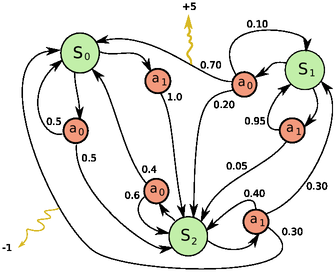
\includegraphics[height=4cm]{images/MDP.png} \\
  \end{figure}
  \end{flushright}
 \end{minipage}
 
 
  Maximiser un critère $ \pi^* \in \operatorname{argmax} = E^{\pi}[r_0 + {\gamma}r1 + {\gamma}^2r_2 + ... ]$
  \newline \hspace*{5.6cm}$ = E^{\pi}[ \sum \limits_{t=0}^\infty {\gamma}^tr_t]$
 
\end{frame}

\note{
Un agent
\newline
Les résultats des actions sont indéterminées
\newline
Pour finir, le problème revient à trouver une politique qui maximise l'espérance des récompenses.
}

\subsection{Apprentissage par Renforcement}

\begin{frame}
 \frametitle{Apprentissage non supervisé}
 \framesubtitle{Apprentissage par Renforcement}

  
  \begin{minipage}{0.4\textwidth}
    \begin{flushleft}
    Algorithmes 
      \begin{itemize}
	\item Sarsa
	\item Q-Learning
      \end{itemize}
    \end{flushleft}
  \end{minipage}
    ~ 
    \begin{minipage}{0.4\textwidth}
    \begin{flushright}
       Q = Etat x Action
      \end{flushright}
    \end{minipage}


    \begin{figure}
  \begin{center}
 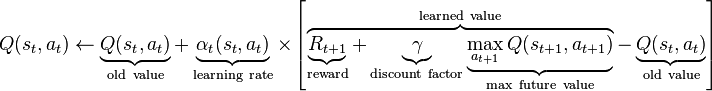
\includegraphics[height=1.5cm]{images/qlearnupd.png} \\
 \end{center}
  \end{figure}
 
\end{frame}

\note{
On s'est concentré sur 2 grands algorithmes : SARSA \& Q-Learning
que nous avons implémenté dans notre bibliothèque

Les 2 utilisent un tableau Q qui permet de facilement retrouver
la meilleur action pour un état donné

La formule de mise à jour durant l'apprentissage est la suivante 

}


\begin{frame}
 \frametitle{Apprentissage par Renforcement}
 \framesubtitle{Prendre en compte l'historique}

     \begin{figure}
    \begin{center}
 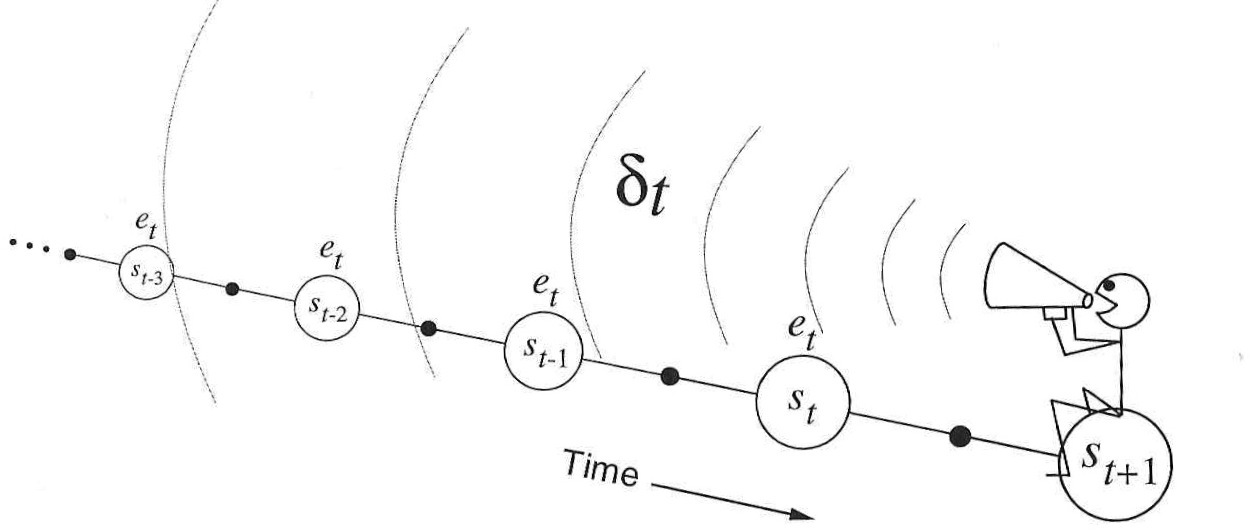
\includegraphics[height=3cm]{images/histo.jpeg} 
 \end{center}
  \end{figure}


      Trace
          \begin{figure}
 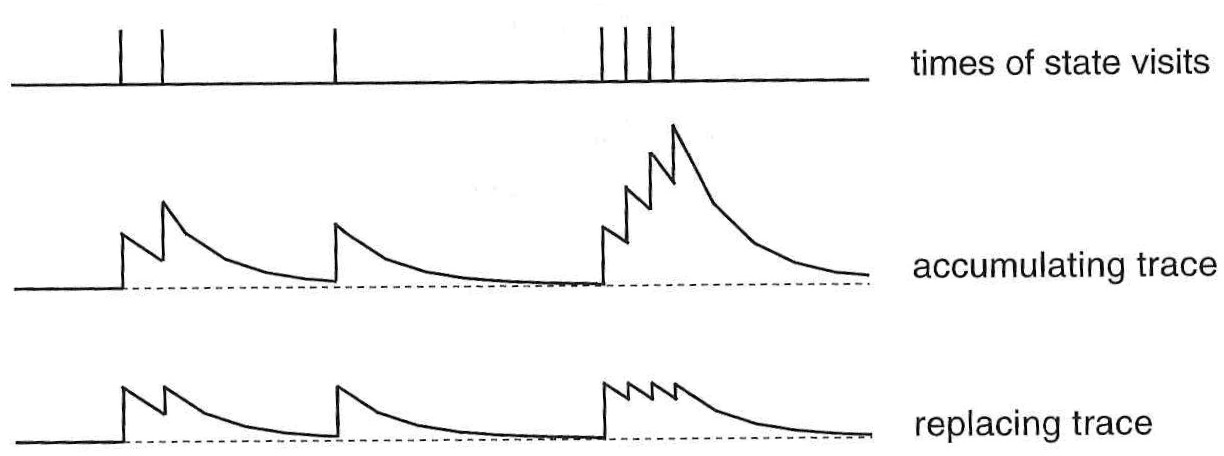
\includegraphics[height=3cm]{images/trace.jpeg}
  \end{figure}

\end{frame}

\note{
Un des problèmes de la version précédente est qu'il n'y a pas de notion d'historique.

Si je fais une erreur ou quelques choses de bien maintenant, c'est uniquement grâce à 
ma dernière action. Ca prolongue beaucoup la phase d'apprentissage.


Mais ça ne suffit toujours pas.
}

\begin{frame}
 \frametitle{Fonction d'approximation}
 \framesubtitle{Descente de gradient}
 
   \begin{minipage}{0.4\textwidth}
    \begin{flushleft}
 Pourquoi? 
 \begin{itemize}
  \item Mémoire
  \item Temps d'apprentissage
 \end{itemize}
    \end{flushleft}
  \end{minipage}
    ~ 
    \begin{minipage}{0.4\textwidth}
    \begin{flushright}
       $Q(s,a) = \sum\limits_{i=1}^n \theta_{i} \times f_{i}(s,a)$
 
      \end{flushright}
    \end{minipage}
 

          \begin{figure}
 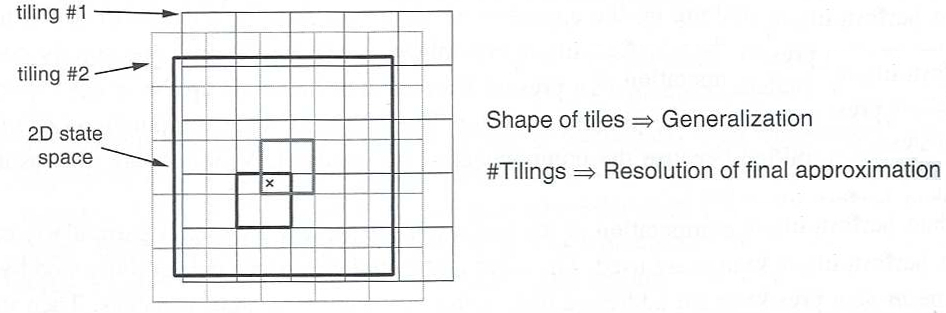
\includegraphics[height=3cm]{images/tiling.jpeg}
  \end{figure}
 
\end{frame}

\note{
l'apprentissage par renforcement «de base» n'est pas extensible à très grand espace d'état, 
car il faut maintenir dans la mémoire très grandes matrices

On va donc chercher maintenant à approximer Q(s,a) par cette fonction.
On notera que les états ne sont alors plus discrétisés.

On gagne en mémoire, plus qu'on tableau teta, et en généralisation, ce qu'il apprend dans
une configuration il peut le généraliser.


Voici qui clos la partie sur l'APR.
}



\begin{frame}
 \frametitle{Semi supervisé}
 
  3 idées 
  \begin{itemize}
   \item Agir sur les récompenses
   \item Agir sur le choix des actions
   \item Agir sur la stratégie (exploitation/exploration)
  \end{itemize}

 
\end{frame}


\note{
Comment intégrer une supervision?\newline
Un tuteur va surveiller l'agent de temps en temps et complémenter la fonction de récompense
\newline contrôler l'agent

}